\documentclass{article}

\usepackage[margin = 2.5cm]{geometry}
\usepackage[bottom]{footmisc} %keeping the footnotes in the end
\usepackage{url} % used for url
\usepackage{graphicx}
\usepackage{caption}
\usepackage{subcaption} % here used for subfigure environment
\usepackage{listings} % used for quoting R code

\setlength{\parindent}{0em}
\setlength{\parskip}{0.5em}
\renewcommand{\baselinestretch}{1.2}

\title{To the rescue of Albanian high school graduates: Predicting admission to public higher eduction institutions programs with a naive estimator and RShiny web application}
\date{\today}
\author{Kreshnik Xhangolli \footnote{Graduate School of Economics, Finance and Management, Goethe University Frankfurt, kreshnik.xhangolli@gmail.com}}


\begin{document}
	\maketitle
	
	\begin{abstract}
		
		We provide an RShiny web application, which enables Albanian high school graduates to use a naive classifier when devising their application strategy for admission in public higher education institutions programs. Our web application has several advantages comparatively to the to the Excel files provided by the Albanian Ministry of Education. (i) Decreases calculation time of applicant's scores from several minutes to miliseconds, (ii) eliminates the possibility of manually inputed mistakes by automating the retrieval of coefficients, (iii) provides a naive estimator that considers the scores of all winners of a program of the last three years and (iv) visualizes the results through data graphs. In addition, to enhance computations speed, we have used a five-levels deep list construct which is saved and called as an RDS.  
		
	\end{abstract}
	
	\vspace{1in}
	
	\textit{Key Words:} RShiny application, Albanian Public Universities, Merit-Preference admission, naive estimator.
	\pagebreak

\section{Introduction}
The admission process to Albanian public higher education institutions (HEIs) is a form of the Gale-Shapley algorithm \cite{gale1962college}. According to Council Decision No 407 of date 1.6.2016 admissions procedures named as \textit{Merit-Preference} are as described in the following \cite{CoM2016}. Students can apply up to ten programs which the student ranks according to her preferences. Students can enroll only in their highest ranked program with a positive admission. Each program ranks applicants based on applicants' scores and admits a predefined quota of highest ranking applicants. If any applicant with a positive admission in a program has another positive admission in another program which she has ranked higher, then the applicants enrolls in the higher ranked program while her position in the lower ranked program is filled with the applicant next in line. The score is calculated with a formula which takes into account students' grade point average, four exams which are divided into two mandatory and two electives, and category of high school. Each program assigns coefficients to all five students' inputs and the list of coefficients is made public before the student selects the elective exams. Applications to the programs are done only after all exams have been graded and the grade has been revealed to the individual student.

This setting means that students face two choices. First they choose the two elective exams and only after the grades for all four exams are realized the students make the second choice of ranking up to ten programs. Assuming rational students, the choice of elective exams would be such that it maximizes students' expected scores for a ranking of desirable admissions, taking in consideration both individual expected performance in the exams and the coefficient assigned by the desirable programs to elective exams. After the realization of the grades, students may revise their list of desirable programs to reflect any mismatch between their expected and real performance in the exams. It is important to note that exam grades are not common knowledge, i.e. each student is aware of her scores only or the scores of other students she can exchange information with - usually with students in the same school. The formula for score calculation is as follows
$$ ([26M + 20(D_1+D_2)]K + 17 (Z_1F_1+Z_2F_2))5 $$
where $M$ represents student's grade average, $D_i, Z_i$ the grades for the mandatory and elective exams and $K, F_i$ program specific coefficient for category of high school and elective exams.

The current tools for score calculation made available from Albanian Ministry of Education (MoE) and Exams National Agency (ENA) are limited to \texttt{pdf} and \texttt{Excel} files. Information on applicants' scores from previous years is found on pdf files usually 500+ pages long. Instead information on coefficients is found on Excel files with 23306\footnote{271 programs $\times$ 86 elective exams} or 9485\footnote{271 programs $\times$ 35 high school categories} rows (table \ref{tb:coeff-calc}). Calculations of scores can be done through another Excel file made available by ENA in which the user is required to manually enter all coefficients and students' inputs (table \ref{tb:points-calc}). Access to the cells and functions is not restricted therefore accidental alternation of the calculating formula is possible. With the tools described above it required us (the authors) on average 6 minutes to calculate the scores for a program. Considering that most high school students do not possess our Excel skills, we can estimate conservatively that a high school students on average would test no more than 5 programs.

\begin{figure}[h]
	\caption{Tools provided by MoE and ENA}
	\centering
	\begin{subfigure}{0.49\linewidth}
		\caption{Excel for point calculation}
		\label{tb:coeff-calc}
		\centering
		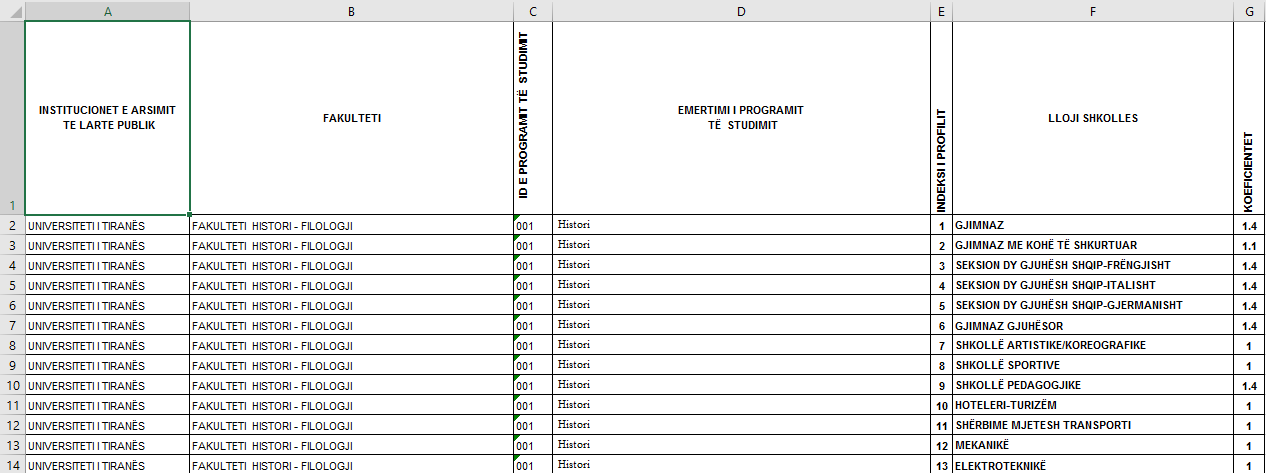
\includegraphics[width=\textwidth]{../Figures/excel_coeff.png}	
	\end{subfigure}
	\hfill
	\begin{subfigure}{0.49\linewidth}
		\caption{Excel for coefficients of schools}
		\label{tb:points-calc}
		\centering
		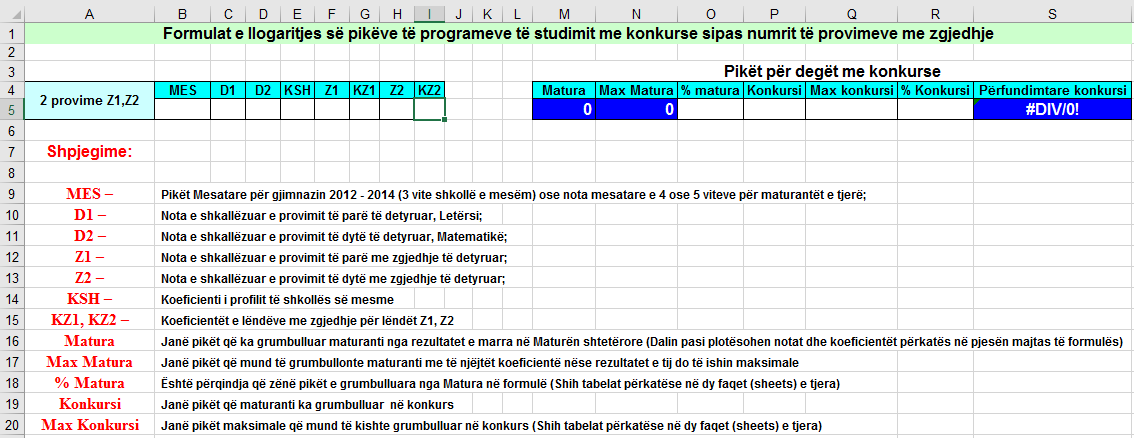
\includegraphics[width=\textwidth]{../Figures/excel_piket.png}
	\end{subfigure}	
\end{figure}

Such severe limitations emphasize the need of better tools for score calculations. This need is made more important considering that 54.8\% of the Albanian youth aged 16 to 27 years old has enrolled or would like to enroll \cite{FES2015}. To our knowledge no such tools are currently available. For the period of 2013-15 an online web application programed in PHP for the calculation of scores was provided as part of a project \footnote{The author Kreshnik Xhangolli was one of the ideators of this project} financed by SOROS Foundation Albania, but which has been currently discontinued. With our RShiny web application we aim to provide Albanian high school graduates with a better tool that not only calculates scores but also provides them with a naive estimator based on percentile calculations. Our web application has several advantages:
(i) decreases calculation time of applicant's scores from several minutes to miliseconds, (ii) eliminates the possibility of manually inputed mistakes by automating the retrieval of coefficients, (iii) provides a naive estimator that considers the scores of all winners of a program of the last three years and (iv) visualizes the results through data graphs. In section 2 we describe some take-ins from the data preparation process. We present the web application in Section 3 and give installation instructions in Section 4.  

\section{Data wrangling}

 We followed good programing practices by breaking up code into scripts which would be called through \texttt{source} if respective dependency variables were not created in the environment. For example:
 \begin{lstlisting}[language=R]
 if (!all(is.element(c("container.rds","programs_list.rds"), 
 		list.files("./RDS")))) source("./F03_embed_lists.r")
 if (!is.element("F02_call", ls())) source("./F02_add_uniques.r")
 \end{lstlisting}
 
We used user-defined functions for data manipulations and computation throughout the project and minimized usage of \texttt{Excel}. In addition we defined a five-level deep \texttt{list} which is stored as an RDS object and called once in the beginning of each RShiny session. As with most real data projects we spent considerate time wrangling with the data; to the extent that we feel ours was a typical 80:20 divide case.

One of the first problems encountered was the table of past applicants scores came in \texttt{pdf} files rather than more data friendly ones. We used open source online tools for converting the tables from \texttt{pdf} to \texttt{Excel} files. The converted \texttt{Excel} tables had an irregular structure in the sense that program and university information was commingled with scores information (figure \ref{fig:irr-records}).

\begin{figure}[h]
	\centering
	\caption{Irregular records}
	\label{fig:irr-records}
	\begin{subfigure}{0.4\linewidth}
		\centering
		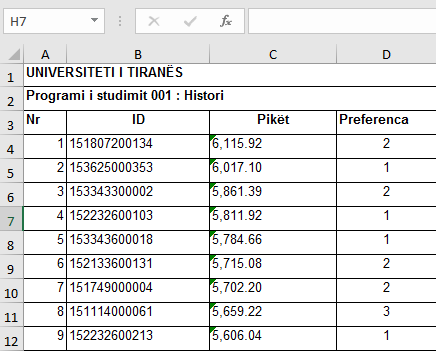
\includegraphics[width=\textwidth]{../Figures/excel_1.png}
	\end{subfigure}
	\hfill
	\begin{subfigure}{0.4\linewidth}
		\centering
		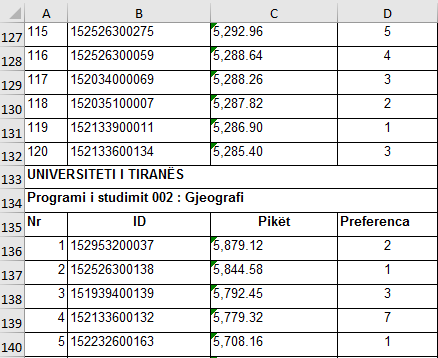
\includegraphics[width=\textwidth]{../Figures/excel_2.png}
	\end{subfigure}	
\end{figure}

Converting the first row with \texttt{as.number} and then discarding the records with \texttt{NaN} first row value could not be used since university and program information could only be retrieved from the current tables. We retrieved the indexes where "Nr" occurred knowing that two sequential "Nr" occurrences would identify a chunk of records with university and program name identified in the two records preceding the first "Nr" occurrence. We iterated through the vector of indexes and copied the respective university and program field for the chunk of records identified by two adjacent indexes. Then we discarded the rows with a \texttt{NaN} first row value after we had converted the row with \texttt{as.number}.

One major difficulty we faced was the usage of non unique program names or codes. As seen from figure \ref{fig:irr-records} the program field is composed of a program code, usually characters ranging from "001" to "303" and the program name. While a program would figure under a certain code in a given year, for example "067", it could be represented with code "072" in another year. In addition even the program names could change in between years, for example from "Arsimi parashkollor" to "Cikel i ulet parashkollor". We decided to retrieve program names for each of the available years using \texttt{dplyr::unique}, create a dataframe with these unique names and save it as a \texttt{csv} file. The \texttt{csv} file was manually manipulated so that each record would hold information only for one program - the names the program was represented in each year and an additional unique name assigned by us. When a program was not offered in a certain year a blank was introduced. We also added a field name reflecting the university which offered the program in the last year. This was necessary since two universities branched off from University of Tirana therefore a program could figure under different universities. Since this attribute is used mainly to subselect program within a university the latest year list of universities was used.

To enhance computation speed, we defined a five level deep \texttt{list}. The data structure (table \ref{tab:container}) reflects the division of the \texttt{container object} into universities, which are divided into the respective programs which are further divided into 3 elements containing past scores, coefficients and the graph object. Past scores are recorded as data frame, coefficients as a list of two data frames and the graph object records a density plot of past scores for the respective university and program. The \texttt{container object} was serialized to an RDS object which is called at each initialization (not computation of scores!) of the web application. This approach results faster since the RShiny session will require only to retrieve the score dataframe, coefficients dataframes and graph object once university and program input is given. This is faster since no filtering or selection of variables will be required to access these three elements.

\begin{table}[h]
	\caption{Five levels deep list}
	\label{tab:container}
	\centering
	\begin{tabular}{l}
		Container: List of N elements (N = number of universities) \\
		\quad .. \$ university: List of P elements (P = number of programs in respective university)\\
		\quad .. .. \quad \$ program: List of 3 element (scores, results, graph)\\
		\quad .. .. .. \quad \quad \$ scores:  dataframe with 2 attributes recording past scores\\
		\quad .. .. .. .. \quad \quad \quad \$ student scores: numeric vector recording student score\\
		\quad .. .. .. .. \quad \quad \quad \$ year: numeric vector recording student year\\
		\quad .. .. .. \quad \quad \$ coefficients: List of 2 elements (dataframes for school and elective coefficients)\\
		\quad .. .. .. .. \quad \quad \quad \$ exams: dataframe with 2 attributes recording exams coefficients\\
		\quad .. .. .. .. .. \quad \quad \quad \quad \$ exam name: character vector recording name of the elective \\
		\quad .. .. .. .. .. \quad \quad \quad \quad \$ exam coefficient: numeric vector recording coefficient for the elective \\
		\quad .. .. .. .. \quad \quad \quad \$ schools: dataframe with 2 attributes recording category coefficients\\
		\quad .. .. .. .. .. \quad \quad \quad \quad \$ school category: character vector recording category \\
		\quad .. .. .. .. .. \quad \quad \quad \quad \$ category coefficient: numeric vector recording coefficient for the category \\
		\quad .. .. .. \quad \quad \$ graph: List holding a Grob (graphical object)\\
	\end{tabular}
\end{table}

\section{RShiny API}
\subsection{Interface}
We designed a user friendly interface for the web application (figure \ref{fig:shiny-interface}). We used the \texttt{sidebarLayout} to divide the input panel (\texttt{sidebarPanel}) from the output panel (\texttt{mainPanel}). Within the input panel we embedded several \texttt{splitLayout} structures to present the input side by side. The input panel requires the user to enter only user specific information such as school type, grades and the program she would like to apply to. This greatly decreases time required to calculate scores and reduces chances of manual mistakes when entering exam or school coefficients. The output panel displays the summary table and the graphs. The summary table displays the numerical value of student's score, the maximal attainable score and the student's percentiles for all years on which there is available data.

Instead the graphs visualize the density functions of past program winners and user's percentile score in the form of partly filled density function. Achieving this type of graph required some programming acrobatics. While getting density plot functions is straightforward with (\texttt{ggplot::geom\_density}), filling the density plot till the user's percentile rank is a trickier. One way to do this is through the (\texttt{ggplot::geom\_ribbon}) which will require the score values in the x-axis and the density value on the y-axis. This required an additional computation step of the density values with \texttt{stats::density}, which returns a dataframe with input and density values. The code below represents the idea \footnote{The code in the script is more complex as we had to adapt it to the \texttt{container} structure. In addition we had to filter the scores for the respective year}. 
 \begin{lstlisting}[language=R]
density.df <- density(scores.df) 
 
ggplot(data=scores.df, aes(x=scores)) + geom_density() + 
	geom_ribbon(data=subset(density.df,scores<score.0),
				aes(ymax = y),ymin=0,fill="grey")
\end{lstlisting}

\begin{figure}[h]
	\caption{Interface of the RShiny web application}
	\label{fig:shiny-interface}
	\centering
	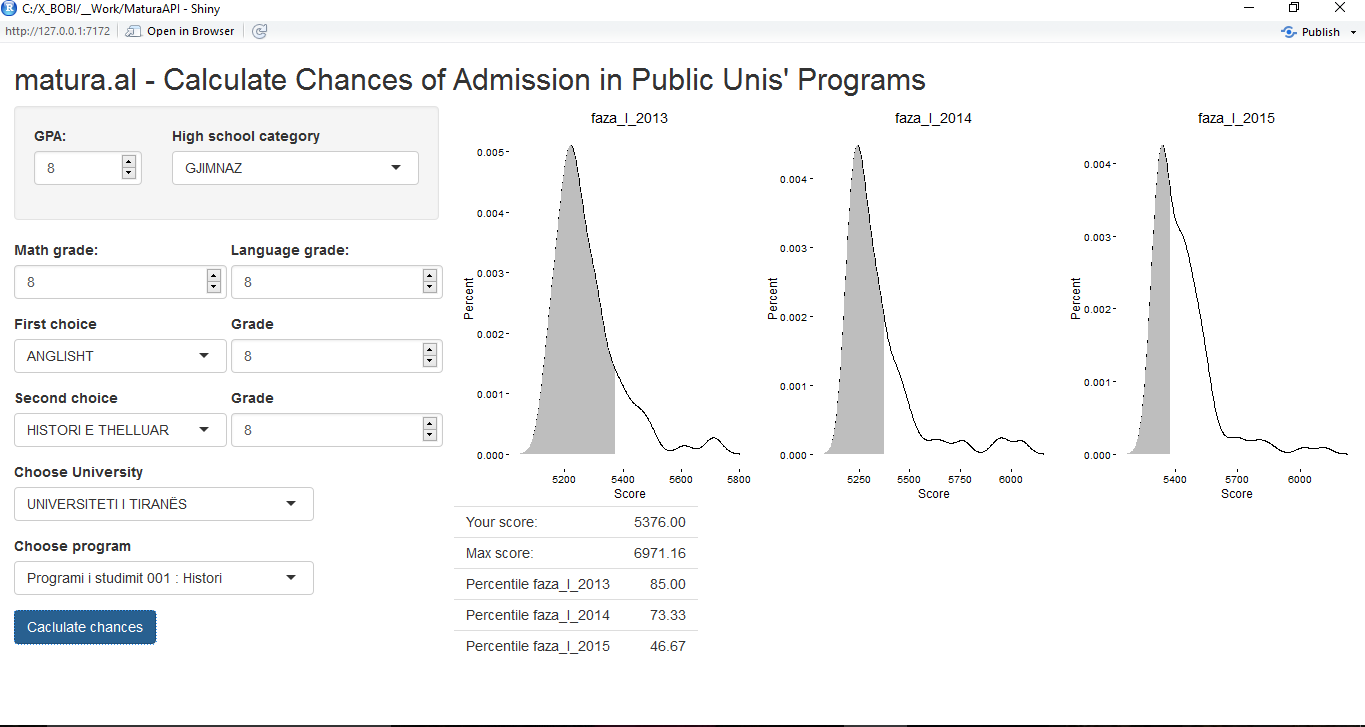
\includegraphics[width=\textwidth]{../Figures/shiny_1.png}	
\end{figure}

We created a series of reactive objects which are computed interactively to any change in inputs. We added a \texttt{submitButton} which introduces a strong control of the application flow, allowing computation only upon button's activation. The \texttt{re\_results} reactive objects would retrieve all information (past scores, coefficients dataframes and plot) for a selected university and program.  A series of other reactive objects would use \texttt{re\_results} to retrieve coefficients and past scores and to calculate scores and percentiles. These latter objects would be combined in reactive plots and tables and linked to output objects. Lastly, to make the selection of programs more user friendly we linked the list box of the programs with that of the universities with \texttt{renderUI}. This means that for any selected universities only respective programs would be displayed for selection. 

\subsection{Naive estimators}

The naive estimator consists of the percentile rank of user's score with respect to respective year past winners. This estimator is calculated for each year on which data is available. Each user can individually then consider how to employ these estimators. Other more simpler classifiers can be employed. For example students can choose to apply for a certain program only if their calculated score is above the min-score of any past years. Other related threshholds would be the maximum min-score or even the average of min-scores. All these classifiers make the implicit assumptions that the preferences and scores of current applicants would be similar to those of previous years. 

We think that doing sensitivity analysis on these estimators is difficult due to the setting of the application process and lack of available data. The game-theory setting adds difficulty since students with high scores can apply to "low scores" program just as an insurance policy. It is not clear whether their scores should be included also in calculating percentile scores. In addition at the current moment we have available data only on winners and not on all applications (scores and ranking of preferences) made in year. We intend to explore predictors under such settings in future research.

\section{Installation}

Making available for non-R users requires usage of chargeable services provided by RStudio server or other providers. We are aware of some other free limited services but we will not opt for them. If such services are contracted then the user of the platform would require only the link of the web application. 

We will provide installation instructions only for R users. Download and unzip the \texttt{zip} file containing project's material. The necessary files to run the application are \texttt{container.RDS} and \texttt{programs\_list.RDS} in \texttt{RDS} folder and \texttt{app.R} under project's root directory. The other files serve for data wrangling purposes and are not necessary if the RDS files are available. Note that one can also copy only the three files in a new folder but the current structure needs to be maintained, i.e. RDS files need to be located in a folder named \texttt{RDS} \footnote{Another option would be to change files path in \texttt{app.R} file}. Package \texttt{Shiny} need to be installed through the \texttt{install.packages(Shiny)} command or by opening \texttt{app.R} and clicking \texttt{Run Application} button, in which case \texttt{Shiny} will auto install. If the latter is chosen, this will also launch the web application. If one would like to use the command prompt to launch the application this is easily done by setting the directory where \texttt{app.R} as the working directory and typing \texttt{runApp()} on the command prompt.

When we make the project public in GitHub and Gist a quick way, assuming package \texttt{Shiny} has been installed, would be by typing

 \begin{lstlisting}[language=R]
 		library(shiny)
		runGitHub("matura-albania-Lite","kreshnikxhangolli")
\end{lstlisting}

% \vspace{1in}
\bibliographystyle{apalike}
\bibliography{biblioMaturaAPI}
	
\end{document}